% !TeX spellcheck = it_IT
\section{5G}

Vengono aggiunti \textit{sempre più casi d'uso diversi tra loro}, e quindi il relativo supporto. Ci sono diversi casi d'uso completamente differenti, come ad esempio:
\begin{itemize}
	\item Multi-hop communication: comunicazione a più salti tra dispositivi per estendere la copertura e migliorare la connettività, utile in ambienti urbani o in aree remote
	\item Device-to-device communication and cooperative devices: comunicazione diretta tra dispositivi senza passare dalla rete centrale, per aumentare efficienza e ridurre la latenza	
	\item Ultra-reliable communication: comunicazioni ad altissima affidabilità, ad esempio per infrastrutture critiche come reti elettriche o trasporti
	\item Massive machine communication: connessione simultanea di un gran numero di dispositivi IoT, tipico di fabbriche smart, logistica e sensori ambientali	
	\item Inter-vehicular/vehicular-to-road communication: comunicazioni tra veicoli e tra veicoli e infrastrutture stradali per supportare la guida autonoma e la sicurezza stradale
	\item Ultra-dense deployments: aree con altissima densità di dispositivi connessi, come uffici o stadi, dove il 5G garantisce prestazioni elevate nonostante l'affollamento.
\end{itemize}
Si ampia il range di frequenze: va da $300MHz$ a $300GHz$. Comprende diverse fasce di frequenza.\\

\newpage

\paragraph{Classificazione International Telecommunication Unit ITU:} Secondo l'ITU le applicazioni possono essere classificate in tre principali categorie di utilizzo:
\begin{itemize}
	\item \textbf{Enhanced Mobile Broadband (eMBB)}
	\begin{itemize}
		\item Servizi orientati alle persone
		\item Elevata banda
		\item HD Streaming, AR/VR
	\end{itemize}
	\item \textbf{Ultra-reliable and Low-latency communication (uRLLC)}
	\begin{itemize}
		\item Servizi orientate alle industrie
		\item Bassissima latenza e affidabilità
		\item Controllo remoto, guida autonoma
	\end{itemize}
	\item \textbf{Massive Machine Type Communications (mMTC)}
	\begin{itemize}
		\item alta densità di connessioni (anche con bassa quantità di dati trasmessi)
		\item smart cities/smart agriculture
	\end{itemize}
\end{itemize}

\begin{center}
	\resizebox{\linewidth}{!}{\renewcommand{\arraystretch}{1.2}
		\begin{tabular}{l | l}
			\textbf{Key Performance Indicator KPI} & \textbf{Minimum Performance Requirement} \\
			\hline
			\multirow{2}{*}{Peak Data Rate} & Downlink: 20 Gbps \\
			\cline{2-2}
			& Uplink: 10 Gbps \\
			
			\hline 
			\multirow{2}{*}{Peak Spectral Efficiency} & Downlink: 30 bps/Hz \\
			\cline{2-2}
			& Uplink: 15 bps/Hz \\
			\hline
			
			\multirow{2}{*}{User-Experienced Rate} & Downlink: 100 Mbps \\
			\cline{2-2}
			& Uplink: 50 Mbps \\
			\hline
			
			5th-Percentile User & Downlink: 0.12 bps/Hz $\approx$ 0.3 bps/Hz \\
			\cline{2-2}
			Spectral Efficiency & Uplink: 0.045 bps/Hz $\approx$ 0.21 bps/Hz \\
			\hline
			
			\multirow{2}{*}{Average Spectral Efficiency} & Downlink: 3.3 bps/Hz $\approx$ 9 bps/Hz \\
			\cline{2-2}
			& Uplink: 1.6 bps/Hz $\approx$ 6.75 bps/Hz \\
			\hline
			
			Area Traffic Capacity & 10 Mbps/m$^2$ (Indoor Hotspot) \\
			\hline
			
			\multirow{2}{*}{User Plane Latency} & 4ms - eMBB \\
			\cline{2-2}
			& 1ms - URLLC \\
			\hline
			
			Control Plane Latency & 20ms \\
			\hline
			
			Connection Density & 1'000'000 devices per km$^2$ \\
			\hline
			
			\multirow{3}{*}{Energy Efficiency} & The support for two aspects: \\
			\cline{2-2}
			& (1) Efficient data transmission in a loaded case \\
			\cline{2-2} 
			& (2) Low energy consumption when there are no data \\
			\hline
			
			Reliability & $1-10^{-5}$ ($99.999\%$) \\
			\hline
			
			Mobility & Up to 500km/h \\
			\hline
			
			Mobility Interruption Time & 0ms \\
			\hline
			
			\multirow{2}{*}{Maximal Bandwidth} & 100 MHz for sub-6 GHz \\
			\cline{2-2}
			& 1 GHz for mmWave \\
			\hline
	\end{tabular}}
\end{center}

Le "direzioni" dell'evoluzione per 5G sono: 
\begin{itemize}
	\item Maggiore spettro
	\item Maggiore efficienza spettrale
	\item Riuso spaziale
	\item "Softwarizzazione" della rete
\end{itemize}

%End L19

\newpage

\subsection{Software Defined Networking SDN}

La struttura di un'applicazione di rete "normale" (senza SDN), consiste di un layer per control e data assieme, il quale si occupa sia del flusso di controllo che del flusso di dati. I dispositivi nella rete hanno al loro interno gli algoritmi di controllo e le regole di forward. \\

SDN "toglie" dai dispositivi di rete la \textbf{parte di controllo}, la quale viene \textbf{centralizzata} in un SDN controller, collegato con tutti i dispositivi e implementa le regole di controllo. Tutte le regole di controllo sono implementati ad un \textbf{livello software} al di sopra del data layer. Offre un'interfaccia unificata all'esterno della rete e permette una conoscenza topologica globale della rete stessa.\\

\begin{center}
	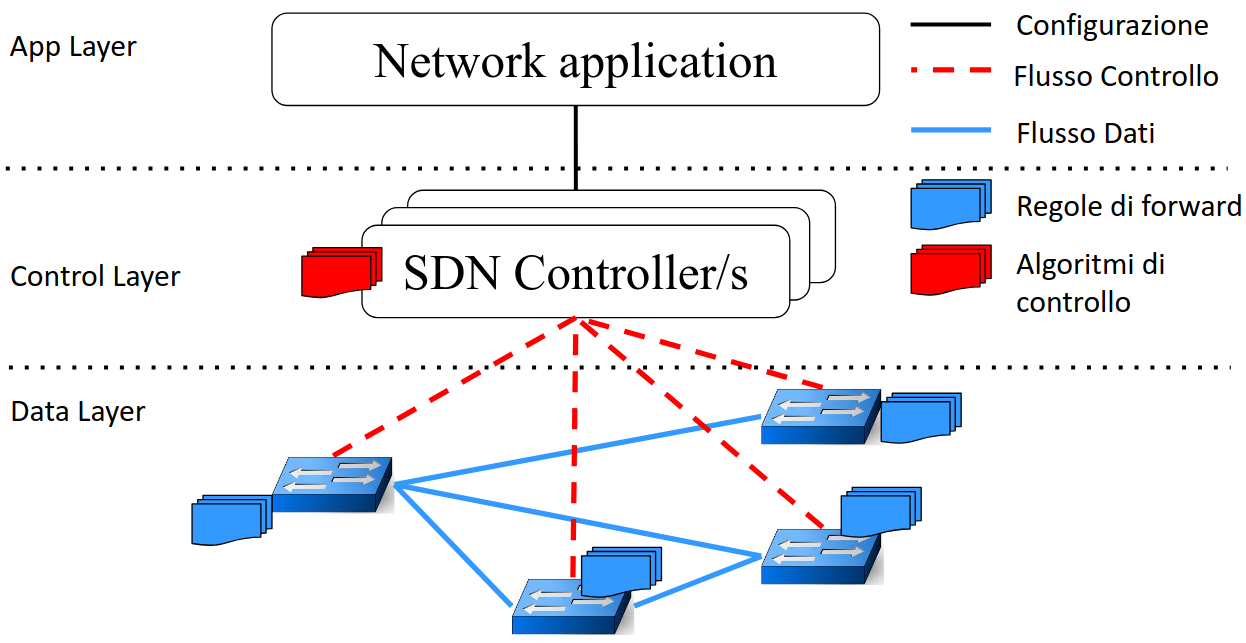
\includegraphics[width=0.8\linewidth]{img/5g/sdn1}
\end{center}

I dispositivi di rete usano un linguaggio in grado di comunicare con l'SDN controller; si ha un linguaggio apposito per la comunicazione tra controller e switch.\\
Si può lavorare anche in maniera reattiva: una volta ricevuto un pacchetto, il dispositivo richiede al controller la regola relativa. In questo modo il controller può inviare/gestire la regola anche per gli altri dispositivi presenti all'interno della rete.\\

Nel networking tradizionale, una volta definiti control e data plane non si possono più modificare i layer, con SDN e fixed-function data plane si possono modificare le funzionalità di controllo a livello software. \\

L'evoluzione vuole andare verso SDN con data plane programmabile, si ha SDN in cui tutto è programmabile, ovvero anche il livello dati ha funzionalità programmabili.
\begin{center}
	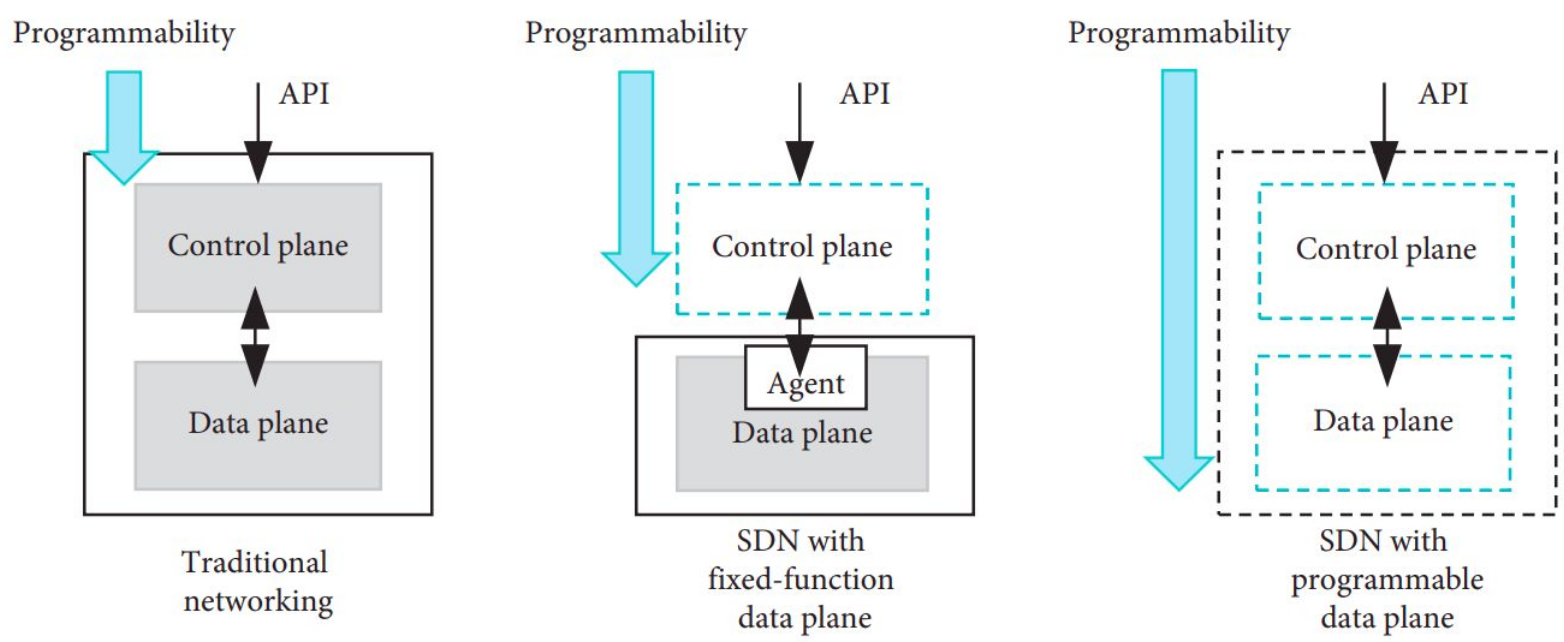
\includegraphics[width=0.85\linewidth]{img/5g/sdn2}
\end{center}
L'architettura prevede una parte di parsing programmabile: si può programmare come il pacchetto ricevuto viene processato. Se data plane è fisso, si possono programmare che regole utilizzare, ma queste devono essere implementate dal data plane, altrimenti nulla. Questo permette molta più flessibilità; le reti cambiano molto velocemente e questo permette di adattare i meccanismi alle condizioni della rete on-the-fly. Si vuole far arrivare il software fino al data link, al bordo del livello fisico.\\

I vantaggi sono diversi:
\begin{itemize}
	\item flessibilità nella gestione della rete
	\item visione centralizzata, quindi ottimizzazione del routing
	\item semplificazione della gestione a livello applicativo (OSS/BSS)
	\item testing e configurazione di nuovi protocolli di rete più semplice e veloce
\end{itemize}

Ma ci sono anche delle sfide: 
\begin{itemize}
	\item i controller diventano un single point of failure
	\item permette di reagire real-time: ma questo deve essere fatto in modo efficiente
	\item ottimizzazione del numero di regole: gestione ottimizzata delle tabelle di forwarding, gestione e garanzia dell'isolamento di reti di overlay (reti logiche), gestione della complessità
	\item sicurezza: controllare il controller vuol dire controllare la rete
\end{itemize}

\newpage

\subsection{Network Function Virtualization NFV}
Prima dell'avvento di questa tecnologia, tutto necessitava hardware dedicato; ogni componente aveva la sua soluzione hardware specifica e la soluzione software corrispondente è strettamente legata.\\

Con NFV si separano le funzionalità hardware e software. Si ha un hardware "standard" sui cui installare l'implementazione software delle funzionalità di rete richieste. Si virtualizza la parte software della funzionalità di rete per poi istanziarla a bordo di hardware standard. Si possono avere istanze in base a dove e quanto necessario.\\ 

Ma come si implementano le funzionalità di rete che implementano il servizio? \textbf{Service Function Chain (SFC)}: grafo delle funzionalità necessarie. \\
Il \textbf{NFV Orchestrator} contiene dei template per delle funzionalità e le istanzia secondo la configurazione necessaria (ovvero in base alla SFC). Si occupa anche di dove metterle (resource allocation); decide dove mettere le istanze necessarie sulle risorse hardware dedicate, in modo che rispettino tutti i vincoli: capacità dei nodi, passaggio, performance, ecc.\\

\subsubsection{Architettura NFV}

Standardizzato da ETSI. La base sono risorse hardware e tramite virtualizzazione vengono offerte risorse virtualizzate. Tutto questo diventa una NFV Infrastructure, ovvero l'infrastruttura su cui instanziare le risorse di rete virtualizzate.\\

Sulla base di questo vengono montate le \textbf{Virtual Network Functions}. Per ogni istanza viene tenuta traccia del suo stato di funzionamento: \textbf{Element Management System (EMS)}.\\

Il tutto si interfaccia alla rete operatore (BSS/OSS) tramite \textbf{NFV MANO} (Management and Orchestration). All'interno della NFV MANO si trovano
\begin{itemize}
	\item \textbf{Virtual Infrstructure Manager (VIM)}: definisce quali risorse sono disponibili e dove
	\item \textbf{VNF Manager (VNFM)}: gestisce le funzionalità di rete istanziate, presenti e future. Collegato al VIM per dire effettivamente \textit{cosa fare}, poi sarà lui che procederà all'istanziazione
	\item \textbf{Orchestrator}: coordina VNFM e VIM. Inoltre è collegato alla rete operatore per ricevere ed orchestrare le richieste all'interno della rete
\end{itemize}

I \textbf{descrittori} sono modelli per i contratti tra le varie componenti del NFV MANO, metadati strutturati che permettono all'orchestrator, VNFM e VIM di sapere cosa fare e come.

\begin{center}
	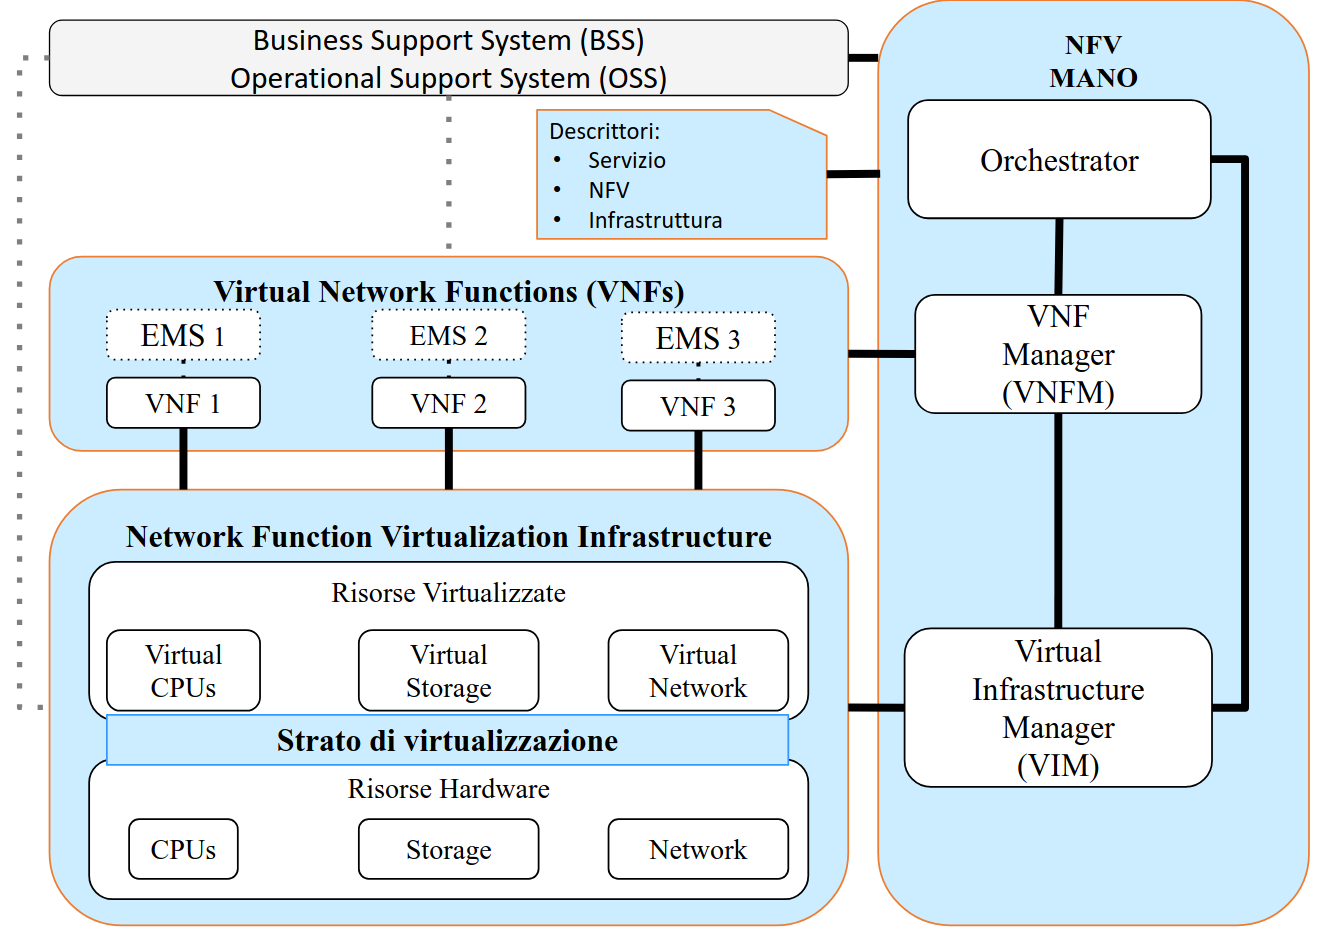
\includegraphics[width=0.8\linewidth]{img/5g/nfv1}
\end{center}

Vantaggi di NFV: 
\begin{itemize}
	\item flessibilità, scalabilità, agilità delle rete e dei servizi; intrinseco nella virtualizzazione
	\item indipendenza hardware e software; si possono modificare senza cambiare l'altro, ad esempio: fixare un bug senza cambiare l'hardware
	\item rapida prototipizzazione e introduzione di nuovi servizi, operatori ed utenti finali
	\item uso delle risorse ottimizzato e condiviso
\end{itemize}

\newpage

Sfide: 
\begin{itemize}
	\item le prestazioni devono essere comparabili con l'hardware dedicato, bisogna garantire certe prestazioni, nonostante l'overhead di virtualizzazione; esistono degli acceleratori, si vuole migliorare il più possibile le VFN, si vogliono usare migliori tecniche di virtualizzazione come Linux Container
	\item gestione efficiente delle risorse: servono tecniche ad hoc per ogni caso d'uso
	\item più software è presente, più problemi di sicurezza possibili esistono
	\item gestione della fase di transizione: devono coesistere hardware e software network function (non possiamo soppiantare la rete istantaneamente)
	\item gestione multi-tenant: più operatori di servizio possono condividere risorse hardware
\end{itemize}

\subsection*{Cloud + NFV + SDN}

5G usa tecnologie Cloud, SDN e NFV.\\

Partendo da un data center (molto) distribuito, si aggiungono le NFV sui vari componenti della rete ed i collegamenti tra questi vengono gestiti tramite SDN controller.\\

\newpage

\subsection{Centralized-RAN C-RAN e Virtual-RAN V-RAN}

La attuale architettura eNodeB è composta da Remote Radio Head RRH e Baseband Unit BBU, questo richiede: 
\begin{itemize}
	\item alimentazione
	\item condizionamento
	\item alto carico computazionale sulla BBU
	\item coordinamento via X2 per ridurre interferenze
	\item limitata visione dello stato degli altri eNodeB
	\item un singolo standard: solo 4G
\end{itemize}

Si può densificare questa struttura? Per ogni antenna bisogna inserire tutte le componenti specificate. Per risolvere questo problema si separano quindi la RRH dai livelli superiori (MAC in su), ponendoli in remoto (ma non troppo remoto, comunque c'è un vincolo geografico, 1km max circa). Si usano delle Virtual Baseband Unit, con sopra tutte le tecnologie necessarie, permettendo anche una migliore gestione in base al carico (virtualizzato).\\

Questo permette:
\begin{itemize}
	\item riduzione CAPEX (capital expenditure): si riduce il numero di apparati e si può riusare il sito, anche per introdurre nuove tecnologie RAT
	\item riduzione OPEX (operational expenditure): minor consumo energetico, ottimizzazione delle risorse BBU remote, gestione dinamica della potenza delle celle
	\item migliori prestazioni: migliore gestione delle interferenze, densificazione delle celle in maniera più sostenibile (dal punto di vista dell'operatore mobile)
	\item Multi-RAT, più tecnologie assieme (in una sola vBBU 3G, 4G e 5G)
\end{itemize}
\begin{center}
	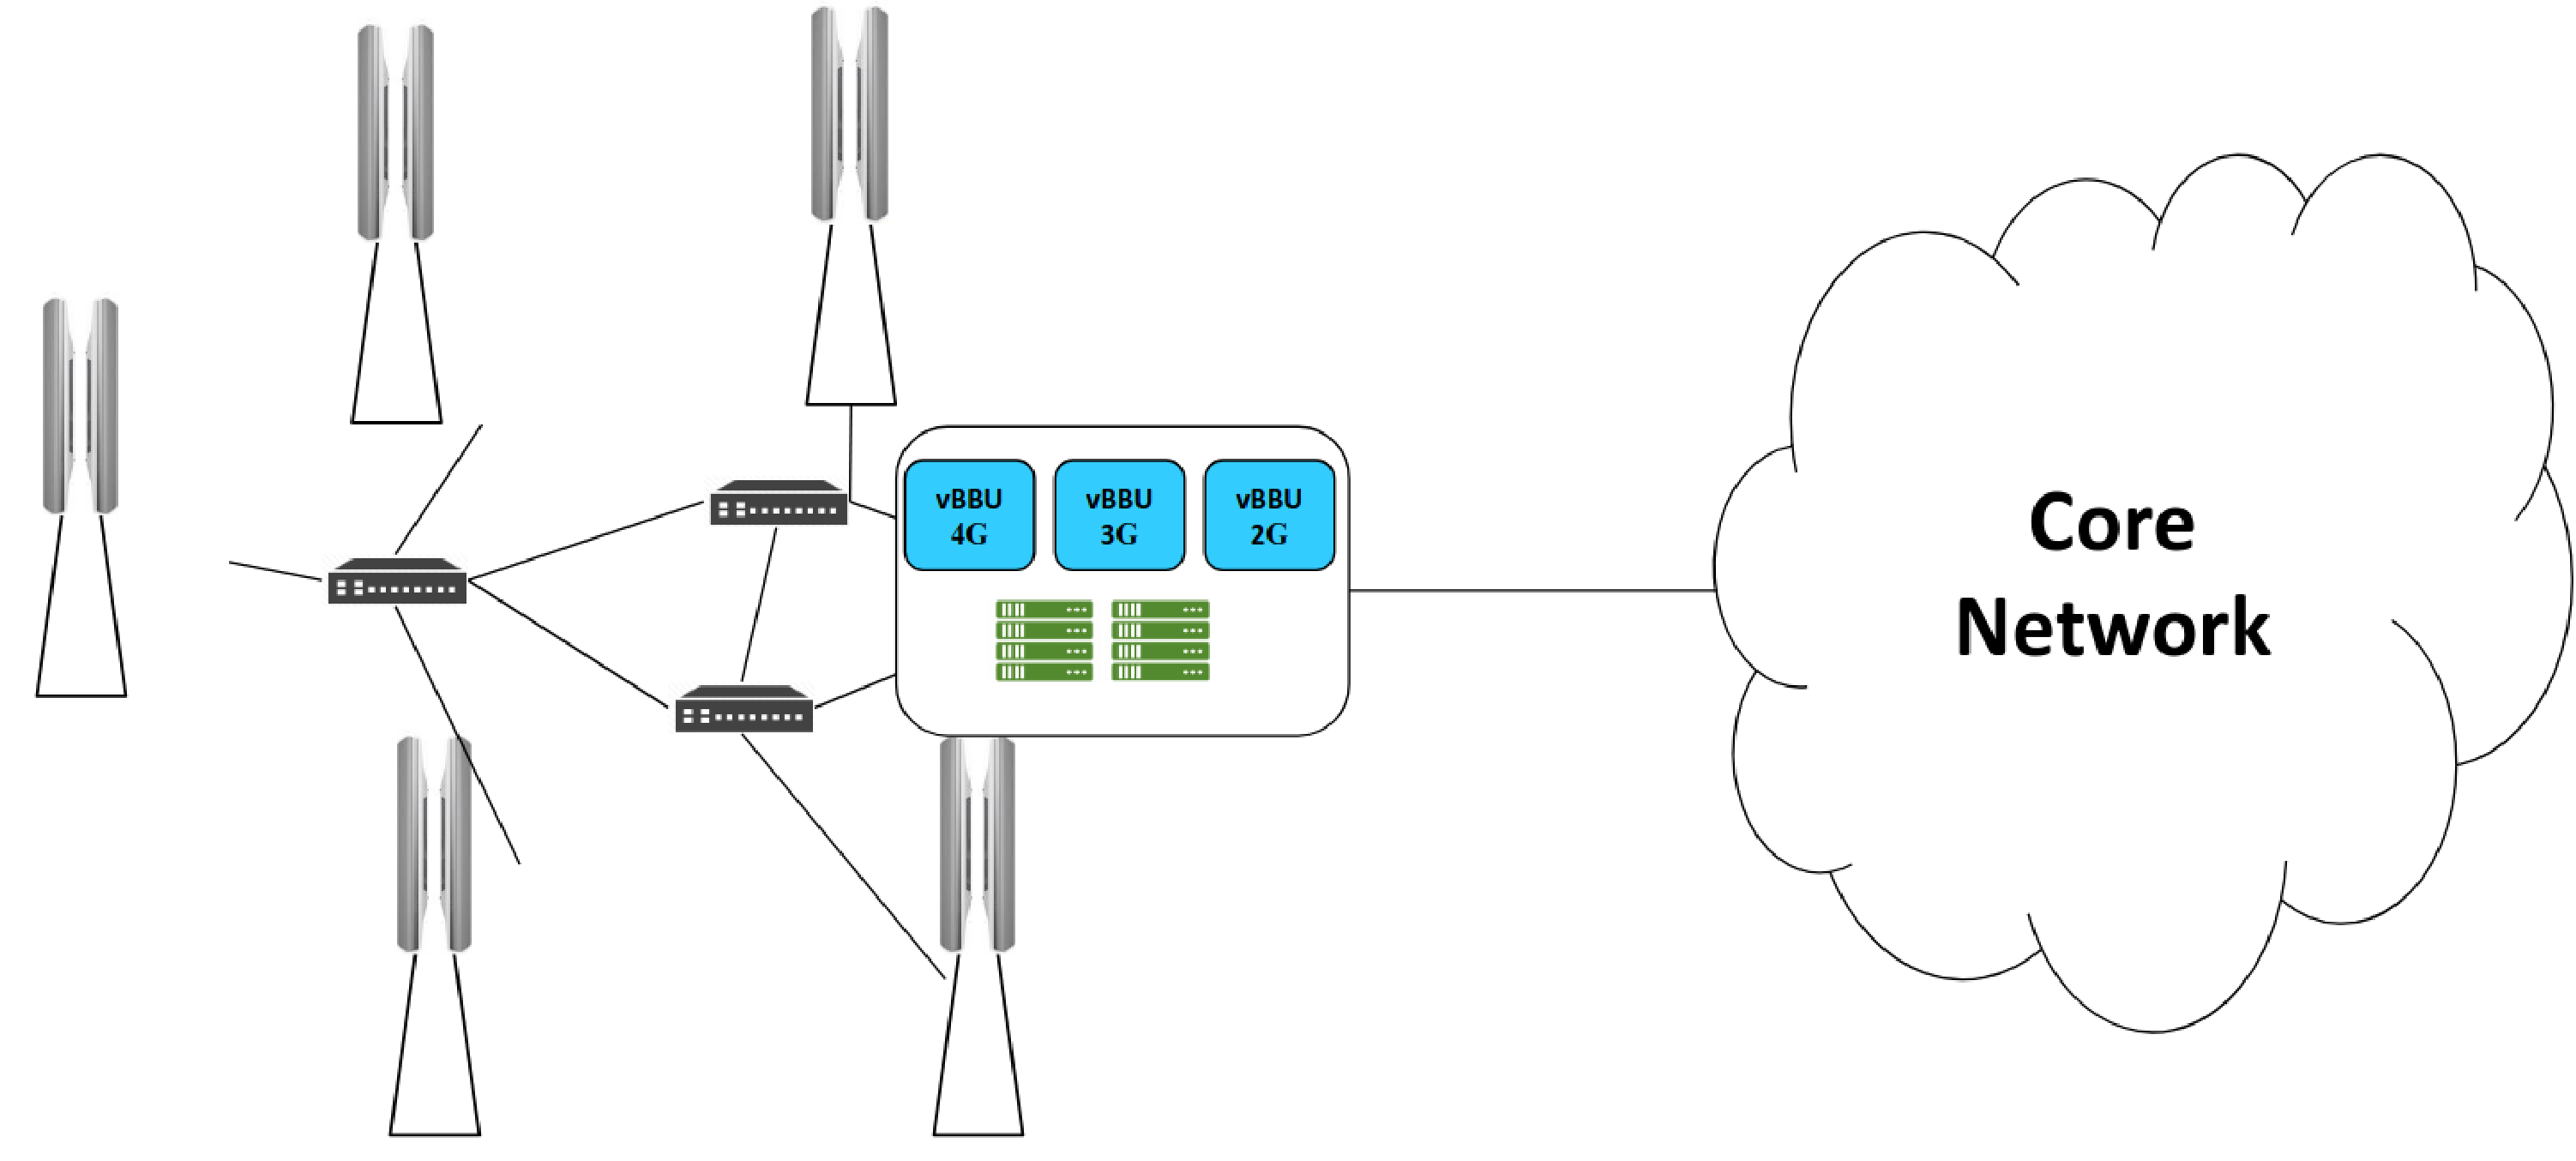
\includegraphics[width=0.98\linewidth]{img/5g/vbbu}
\end{center}

Per scalare la rete: si possono installare nuove RRH, senza dover aggiungere BBU, al posto della quale è necessario solo scalare orizzontalmente la vBBU già esistente (permetterne più istanze in parallelo, i.e., aumentare le performance). Tramite un singolo data center si possono gestire molte BS, risultando in una migliore gestione.\\

\subsection*{Cloud Computing}
Dai, sai come funziona, \href{https://it.wikipedia.org/wiki/Cloud_computing}{\texttt{ma nel caso}}. Una struttura tipica:
\begin{center}
	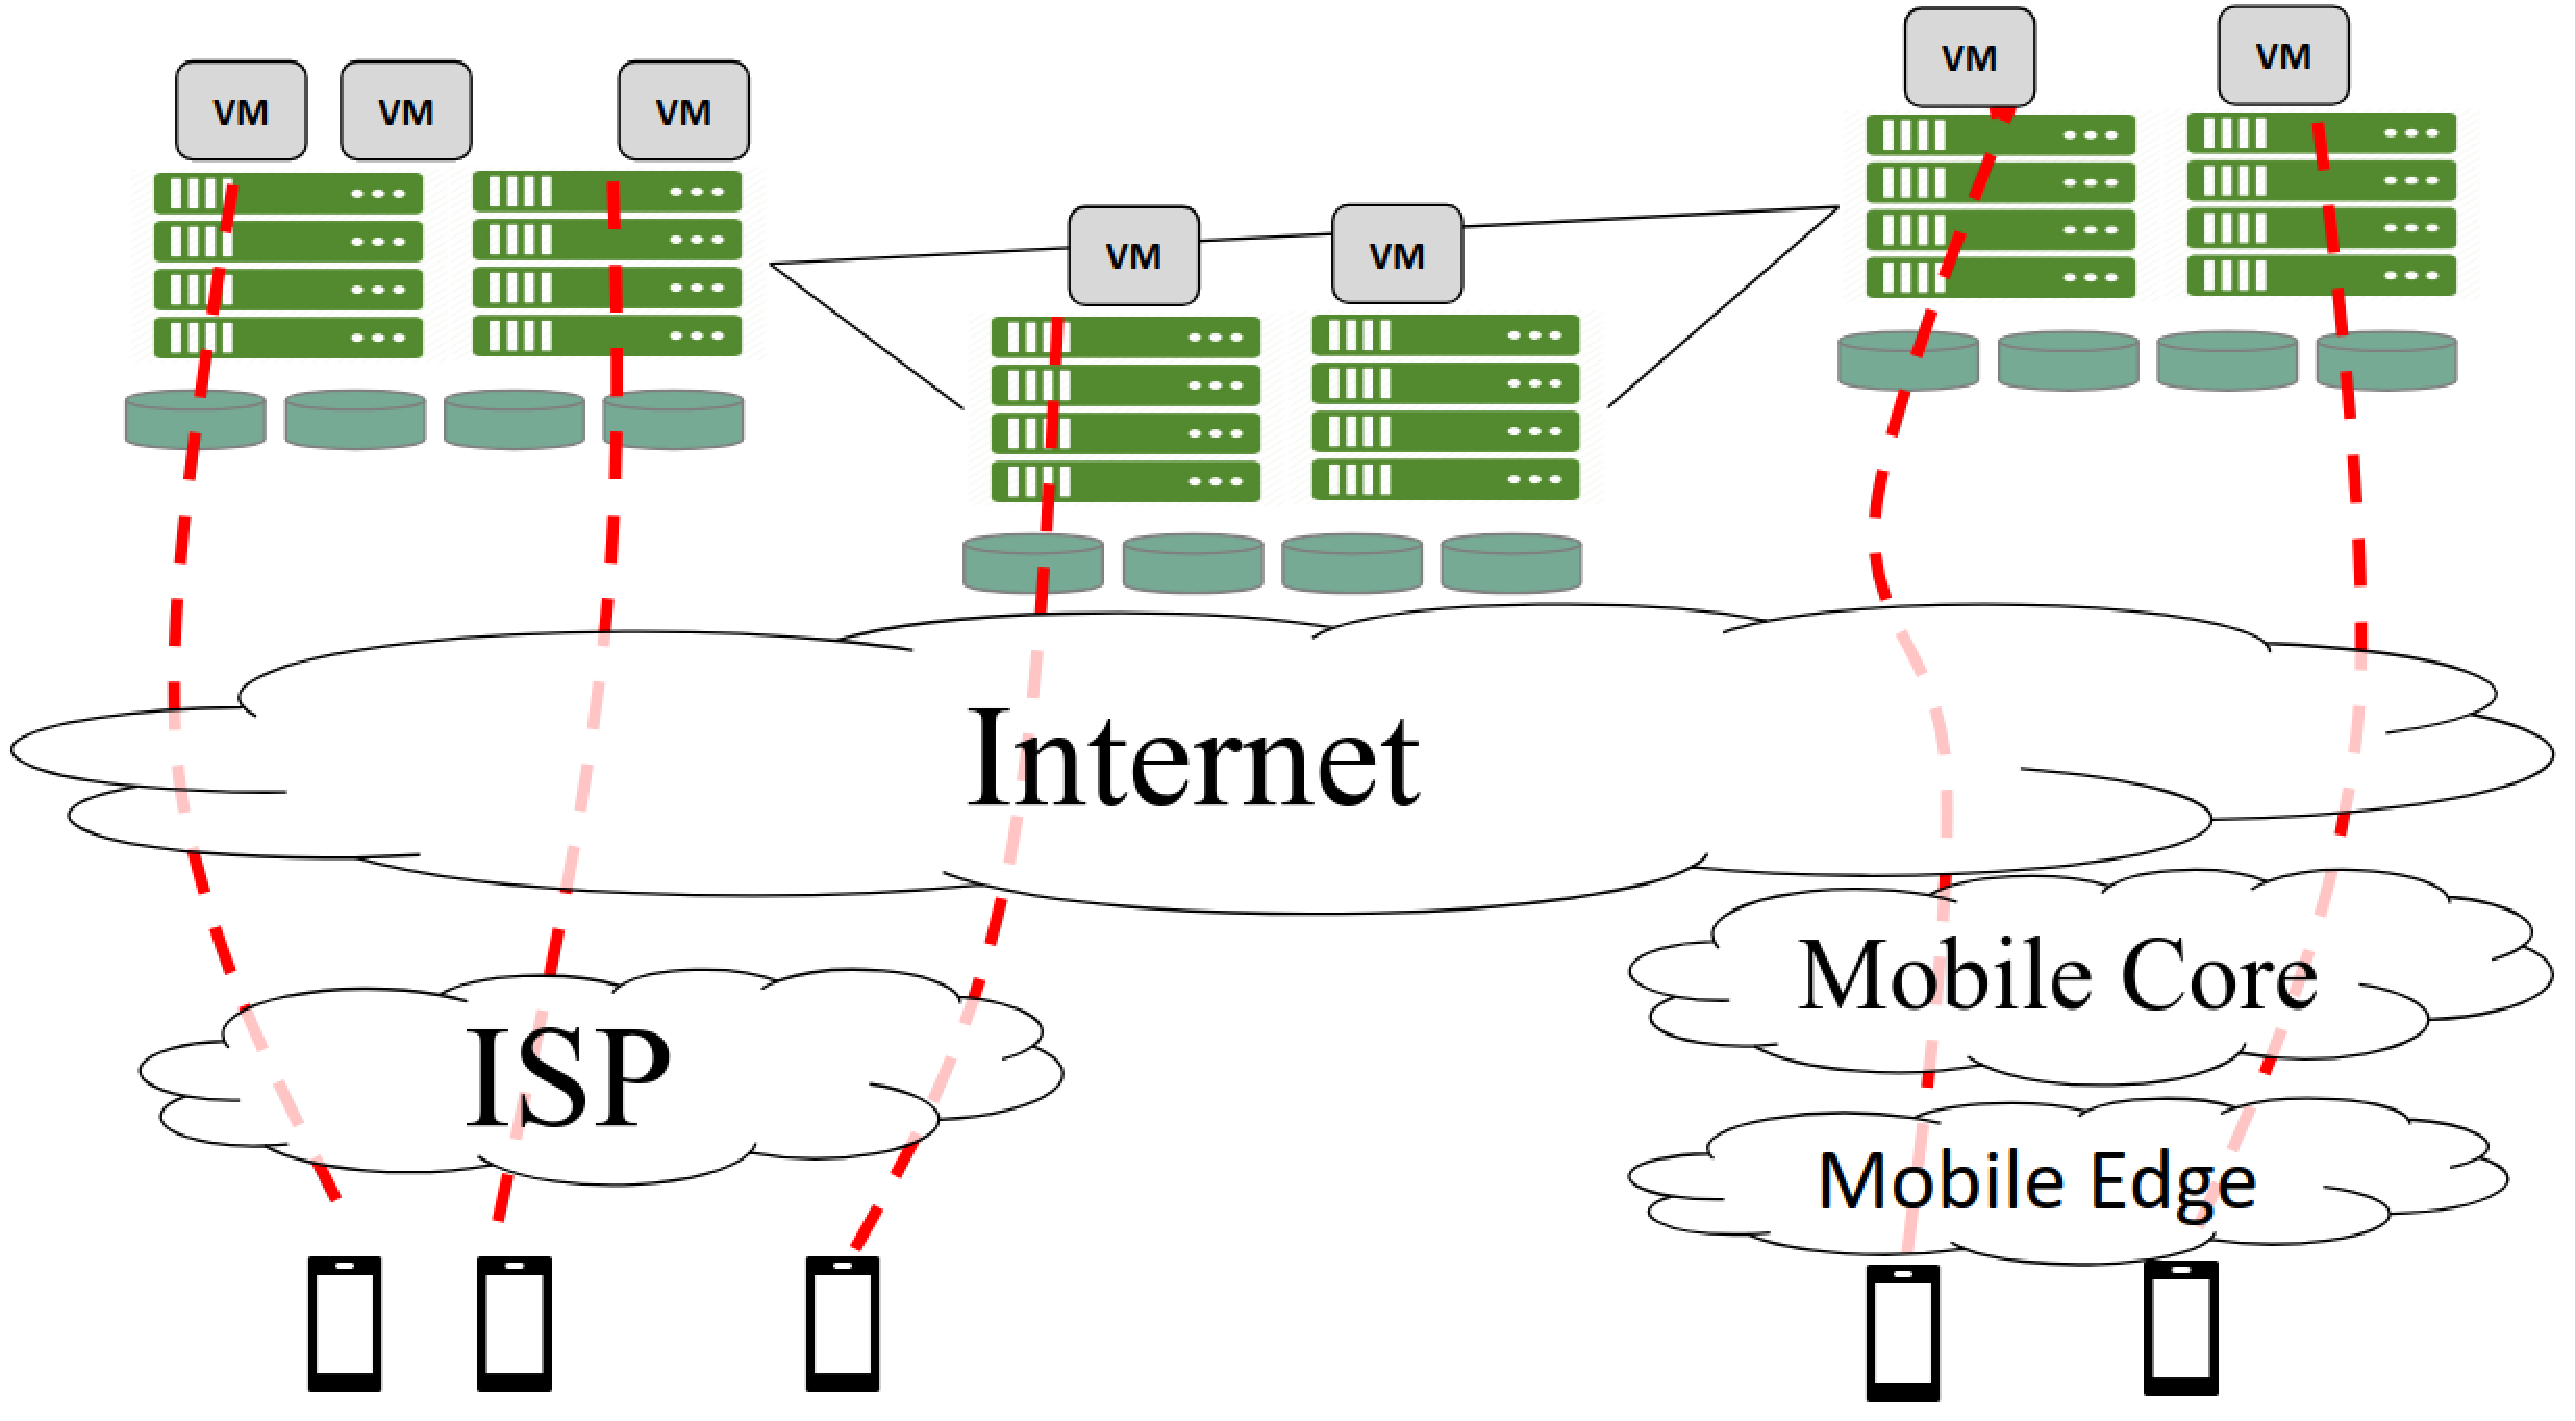
\includegraphics[width=0.8\linewidth]{img/5g/clud}
\end{center}
Questo potrebbe avere (relativamente) elevata latenza per i servizi, elevato jitter (deviazione standard sul delay alta), applicazioni near real-time sono difficili da realizzare.

\newpage

\subsection{Mobile Edge Computing MEC (ETSI)}

Mobile Edge Computing (chiamato anche Multi-access Edge Computing). Si vuole avere delle risorse computazionali il più vicino possibile all'utente. 
\begin{center}
	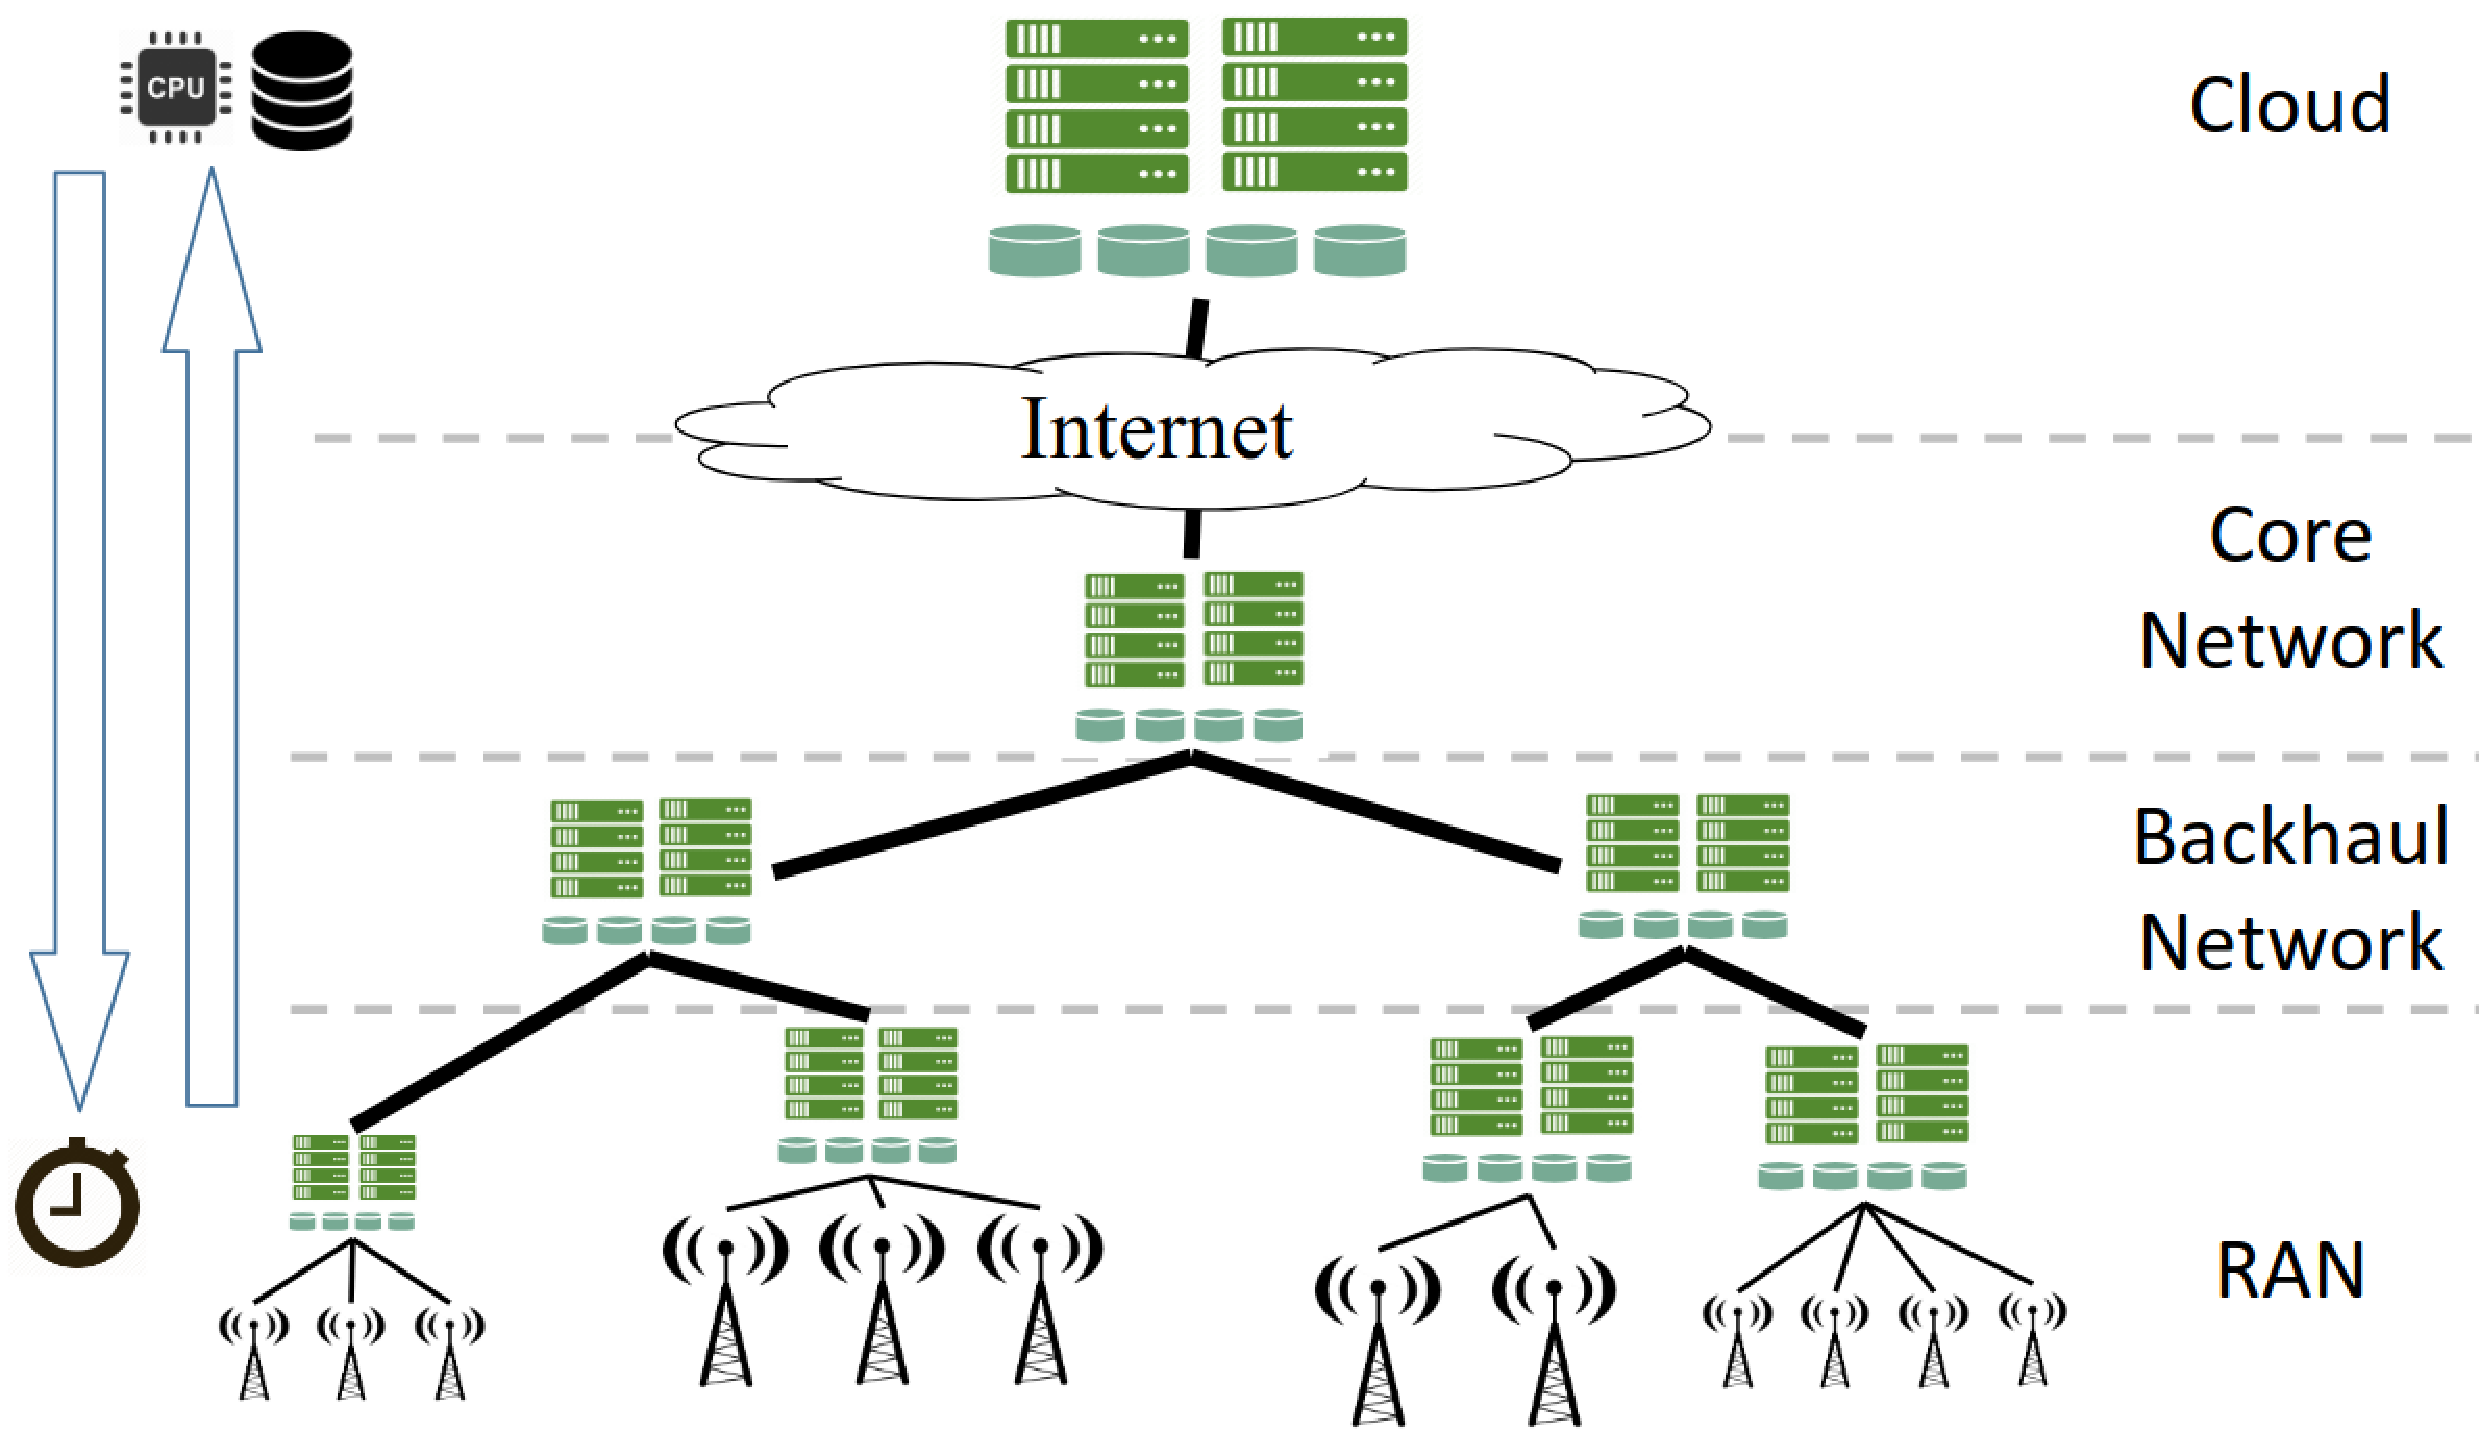
\includegraphics[width=0.9\linewidth]{img/5g/mec}
\end{center}
Si hanno risorse ad ogni livello (Cloud Edge Continuum), ovviamente con limitazioni su applicazioni contenute e capacità disponibile.\\

Le domande sono: 
\begin{itemize}
	\item Dove installare i vari moduli? Cloud? MEC server? Dispositivo stesso? 
	\item Come viene gestita la mobilità dei dispositivi che utilizzano il servizio?
\end{itemize}
La risposta dipende dai requisiti del modulo e dei link di comunicazione tra moduli.\\

Vantaggi: 
\begin{itemize}
	\item Architettura fortemente decentralizzata e localizzata
	\item Riduzione della latenza e jitter end-to-end
	\item Riduzione traffico verso il core della network
	\item Miglior support a Servizi Location/Context-Aware
\end{itemize}

\newpage

Sfide: 
\begin{itemize}
	\item Integrazione nella rete: Come coesistono MEC e standard 3GPP? Come garantisco la trasparenza a UE?
	\item Portabilità delle applicazioni MEC, Allocazione e de-allocazione trasparenti ed impercettibili (seamless); Architetture HW e SW standard e open
	\item Sicurezza; Come garantisco isolamento tra le VM nei MEC server? Come controllo dinamicamente l'uso corretto delle risorse
	dell'operatore?
	\item Performance; Dimensionamento delle VM; Allocazione ottimizzata delle VM all'interno della rete
	\item Resilienza
\end{itemize}

\subsection{Network Slicing}

Network slicing è un concetto che trasforma la rete/sistema  da \textbf{paradigma} statico ad uno \textbf{dinamico} (nei primi standard si avevano qualità di servizio predefinite, qualunque fosse il servizio), nel quale \textbf{reti logiche} vengono create \textbf{on demand} con risorse e topologie ottimizzate per servire uno scopo specifico, una categoria di servizi o singoli utenti.\\

\textbf{Network Slice Instance} è un insieme di network function e risorse di rete organizzate e configurate per fornire una rete logica che soddisfa certe caratteristiche.\\

Per ogni classe di servizio/esigenza viene costruito un overlay di rete ad hoc al di sopra della rete fisica. Diventa molto più flessibile la gestione della rete \textit{al servizio di un servizio}, viene creata una slice della rete ad hoc per il servizio.\\

5G abbandona l'idea degli standard precedenti in cui \textit{one size fits all}, si hanno diversi casi d'uso e le risorse vengono allocate di conseguenza. \\

%End L20

\newpage